\documentclass[../Article_Model_Parameters.tex]{subfiles}
\graphicspath{{\subfix{../Figures/}}}
\begin{document}
	
	\label{CH: Experiments}
	
	In order to solve the optimization problem presented by Equation \ref{EQ: Optimization_formulation_MLE}, it is necessary to have knowledge of the dataset ${\color{black}Y}(t)$, which was obtained by extracting oil from chamomile seeds. The experiments were performed by \citet{Povh2001}. To prepare the seeds for extraction, they were first pre-treated using a knife mill (TECNAL, model TE 340) to reduce their particle size. The mean
	particle diameter was determined by the Sauter equation and is equal to $0.3\times 10^{-3}$m. The actual density of the chamomile particles was measured through helium pycnometry at the Institute of Chemistry IQ/Unicamp's Analytical Facilities. The bulk density of the bed was computed based on the feed's mass and the extractor's volume. The total porosity of the bed, including the particles, was determined using the following calculation: $\epsilon=1-\frac{d_a}{d_r} = 1-\frac{370}{1364} = 0.73$.
	
	%The moisture content of the seeds was then determined using an Infrared Moisture Analyser, which revealed an average moisture content of 4.83\% in the solid particles after grinding. Next, the density of the solid material was measured using a pycnometer, which can be found in Appendix \ref{CH: Solid_Density_Measurment}. Finally, the material's porosity was also calculated to be 0.5, as explained in Appendix \ref{CH: Porosity}.
	
	The experiments were conducted using an extractor with diameter of $3.96\times 10^{-2}$ m and length $16.55\times 10^{-2}$ m. Twelve experiments were performed under different but constant in time operating conditions: $30-40^\circ C$, $100 - 200$ bar, and $1.33-6.66 \times 10^{-5}$ kg/s. The amount of solid material used for extraction was $75\times 10^{-3}$ kg, which was sufficient to fill the whole vessel. Samples were collected every 30 min for the first 3 h and every hour afterwards up to 10 h. 
	
	%After loading the material into the extraction chamber, the extractor was pre-heated to the desired temperature. The outlet line was then closed, and the extraction chamber was filled with $CO_2$. The $CO_2$ was pumped and compressed until the desired operating pressure was reached. When the operating temperature and pressure were achieved, the outlet line was opened, allowing the solvent to flow through the system. The solvent extracted the essential oils from the solid material, and the resulting $CO_2$ and oil mixture flowed from the extractor to the separator. The separator operated at $50^\circ C$ and $50$ bar. The gaseous $CO_2$ exited from the top and was recycled to the $CO_2$ storage tank. The oil stayed at the bottom of the separator in the liquid form. The extraction time for each batch was 150 minutes, measured from the opening of the extractor outlet port. Every 5 minutes, the oil was drained from the separator, and its weight was measured. The resulting time series ${\color{black}Y}(t)$ corresponds to the output of measurement Equation \ref{Model_measurment_1} and can be used for parameter estimation.
	
	\begin{figure}[!h]
		\centering
		\begin{subfigure}[b]{\columnwidth}
			\centering
			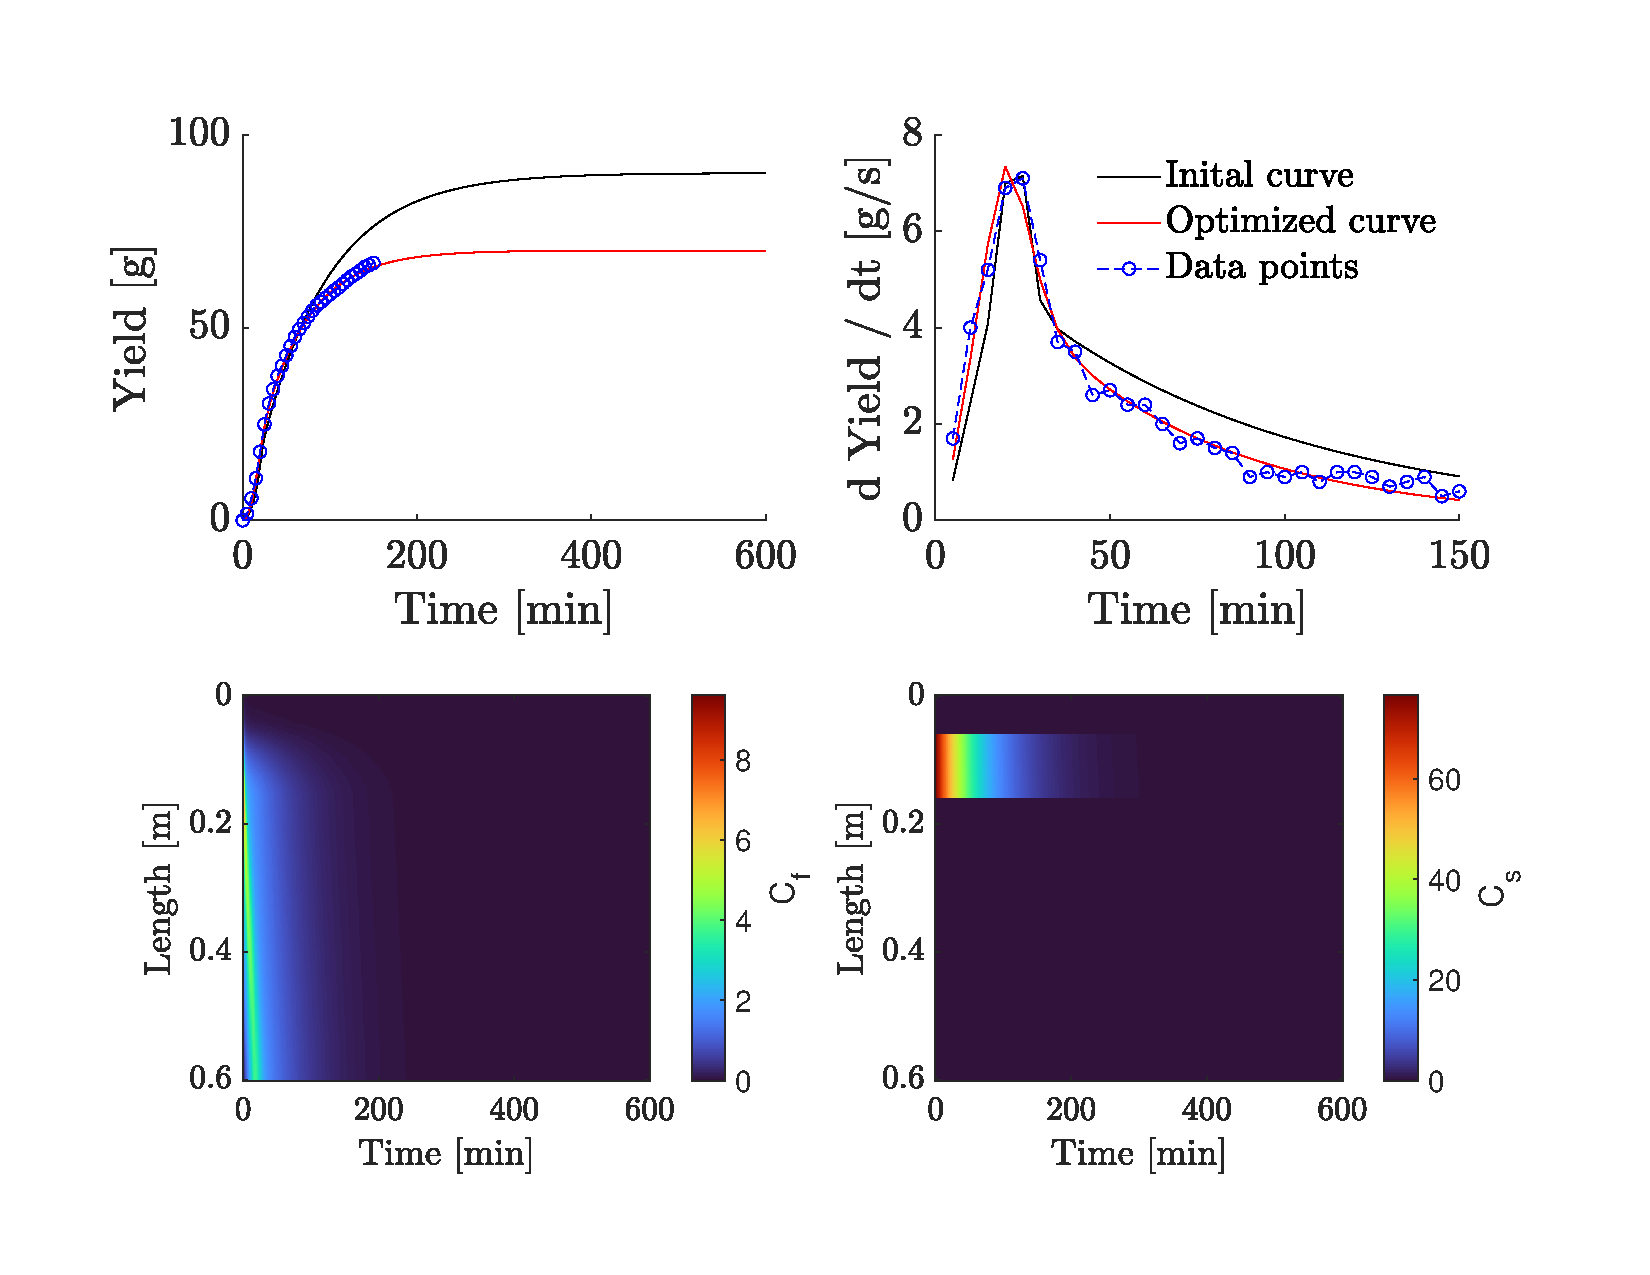
\includegraphics[trim = 2cm 10.5cm 2.5cm 1.7cm,clip,width=0.99\textwidth]{/Results_estimation/Fitting_LUKE_T40_P200.pdf}
			\caption{Experiment at $40~^\circ C$ and 200 bar}
		\end{subfigure}
		\begin{subfigure}[b]{\columnwidth}
			\centering
			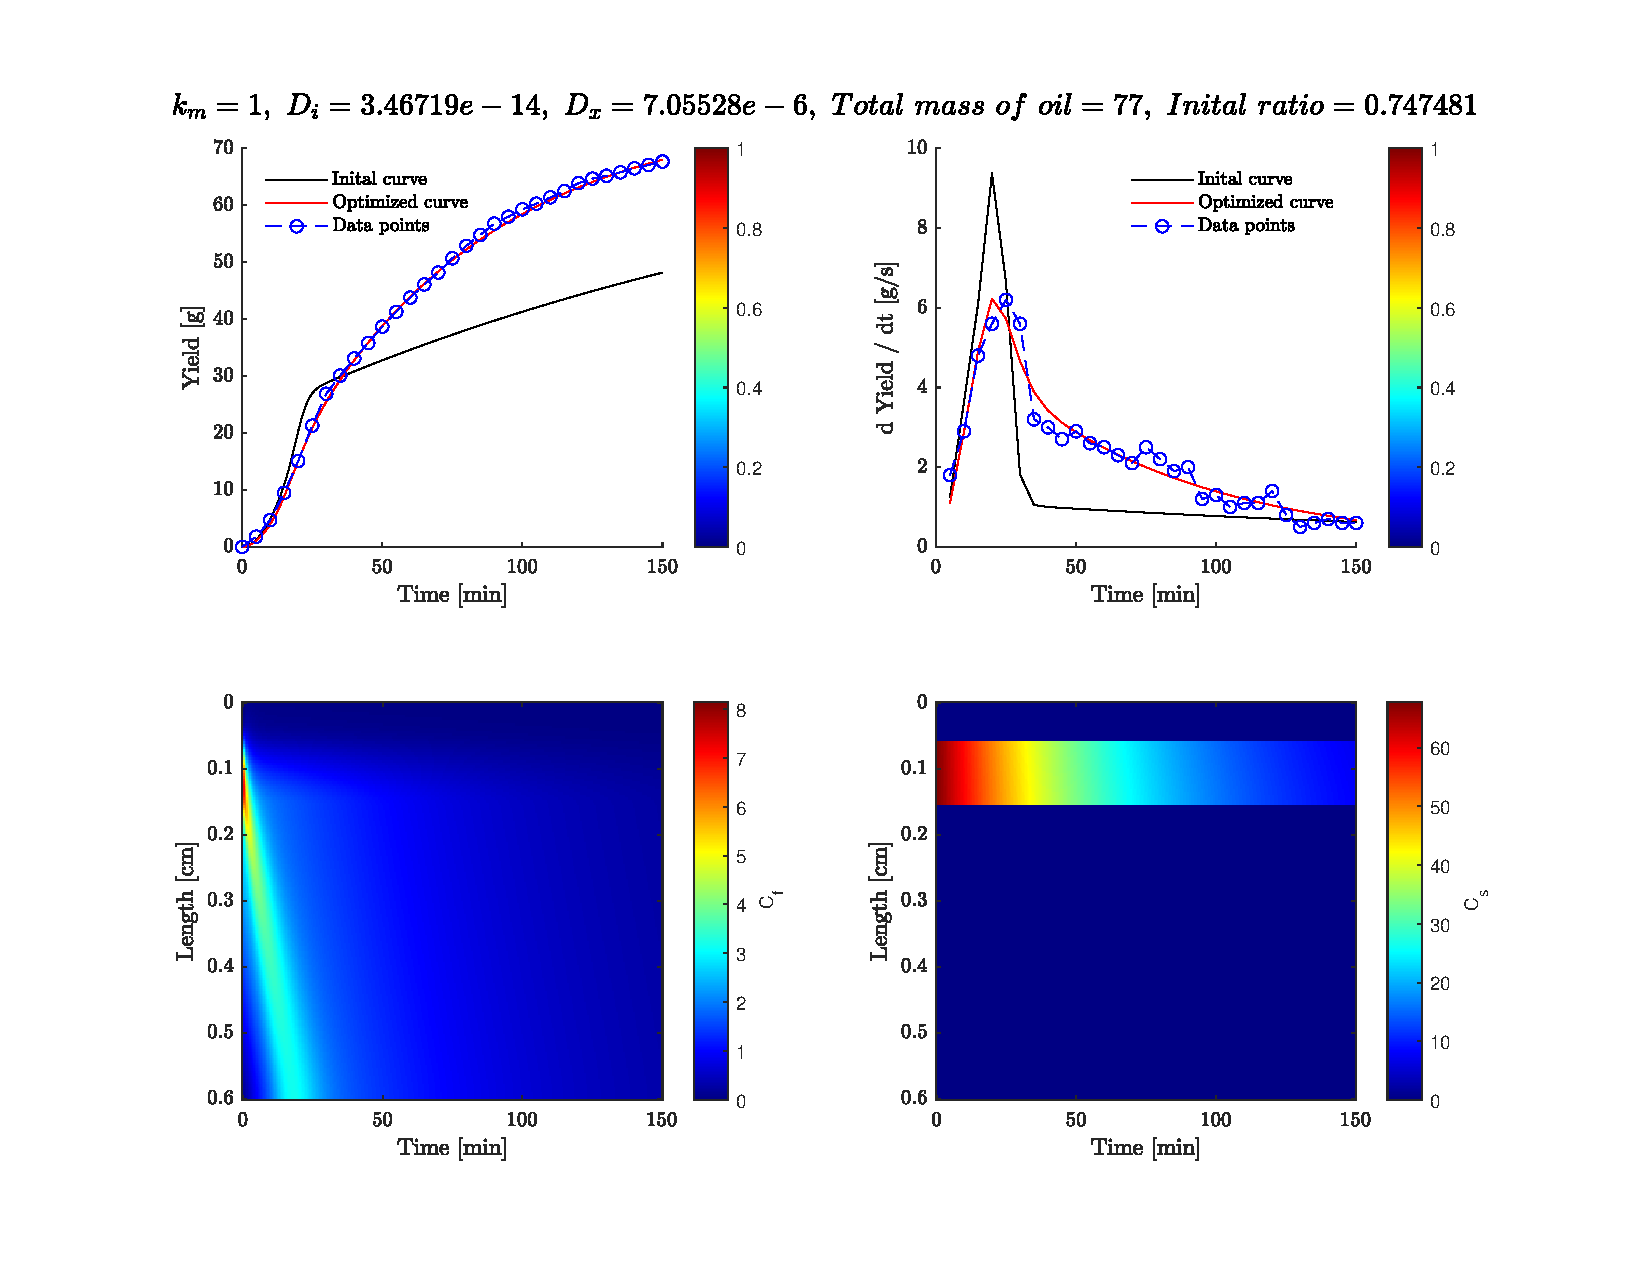
\includegraphics[trim = 2cm 10.5cm 2.5cm 1.7cm,clip,width=0.99\textwidth]{/Results_estimation/Fitting_LUKE_T50_P200.pdf}
			\caption{Experiment at $50~^\circ C$ and 200 bar}
		\end{subfigure}
		\hfill
		\begin{subfigure}[b]{\columnwidth}
			\centering
			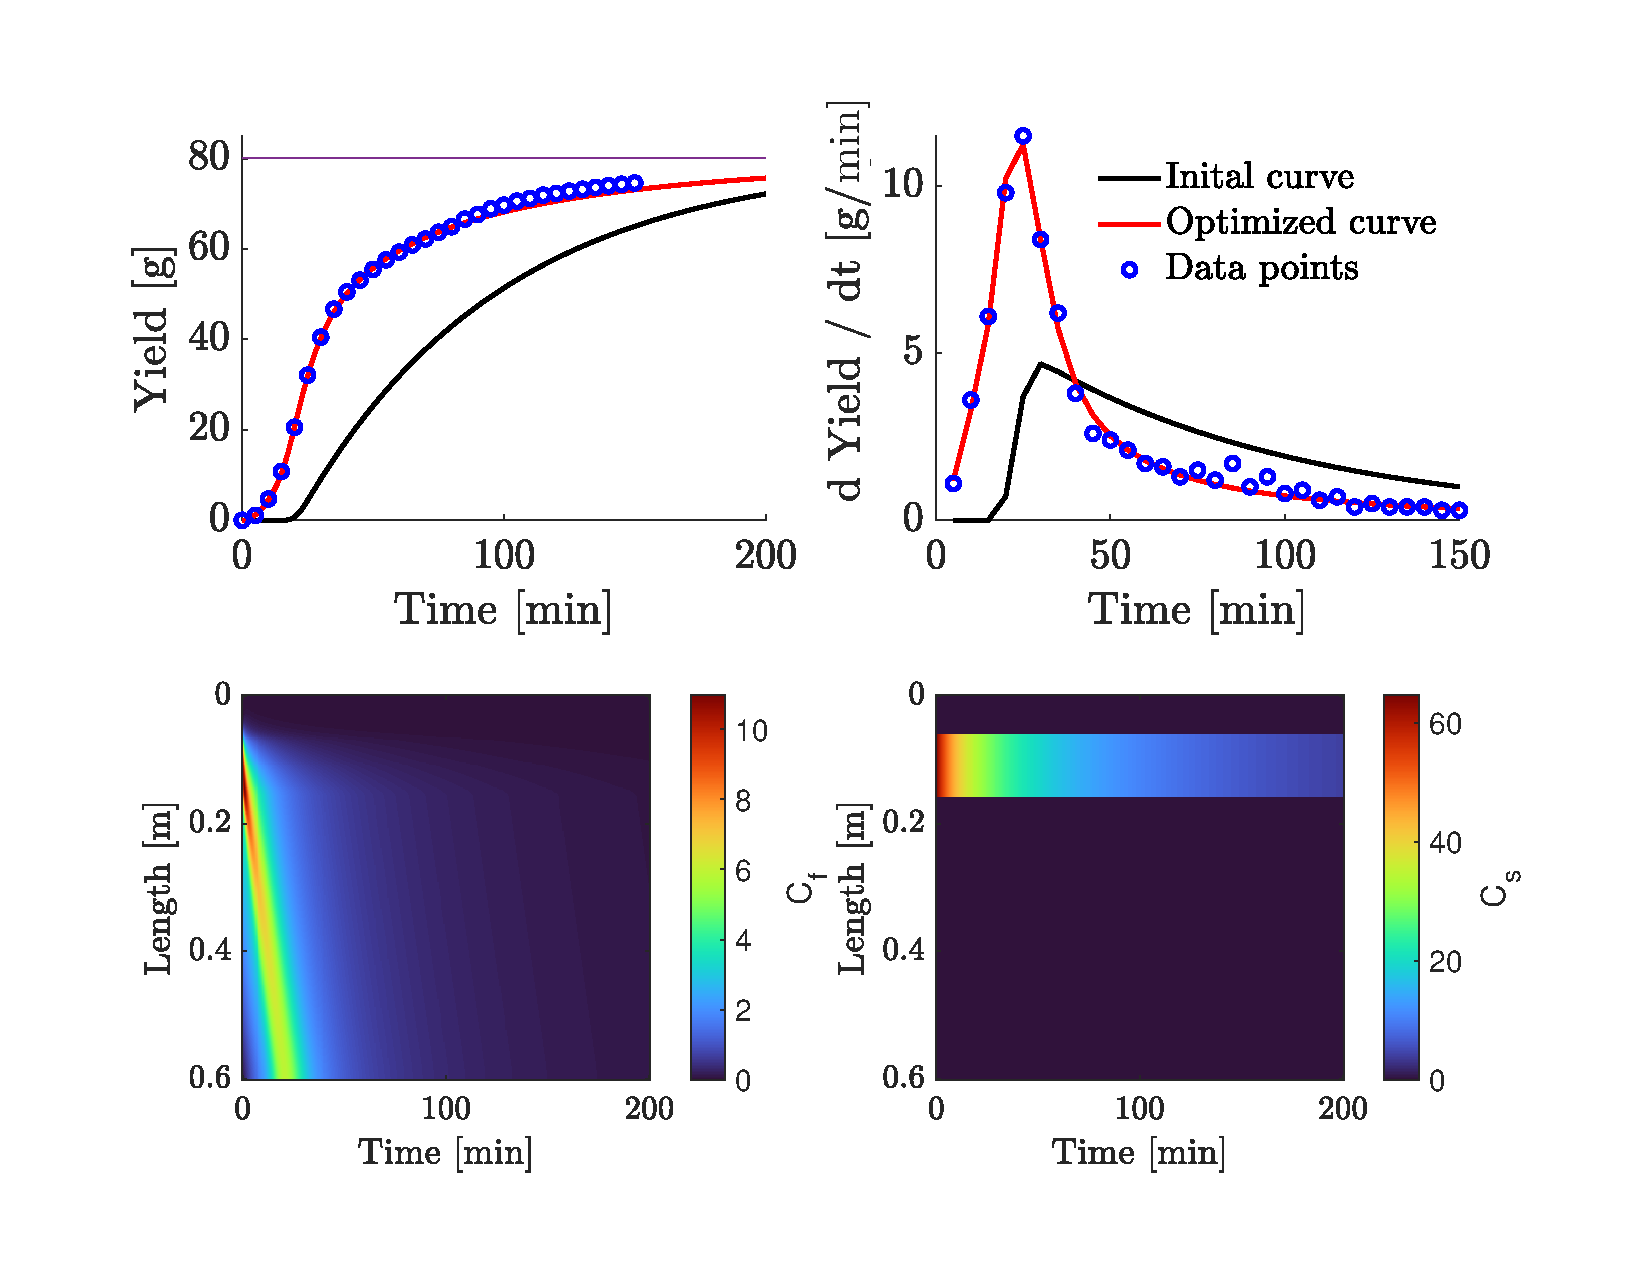
\includegraphics[trim = 2cm 10.5cm 2.5cm 1.7cm,clip,width=0.99\textwidth]{/Results_estimation/Fitting_LUKE_T40_P300.pdf}
			\caption{Experiment at $40~^\circ C$ and 300 bar}
		\end{subfigure}
		\begin{subfigure}[b]{\columnwidth}
			\centering
			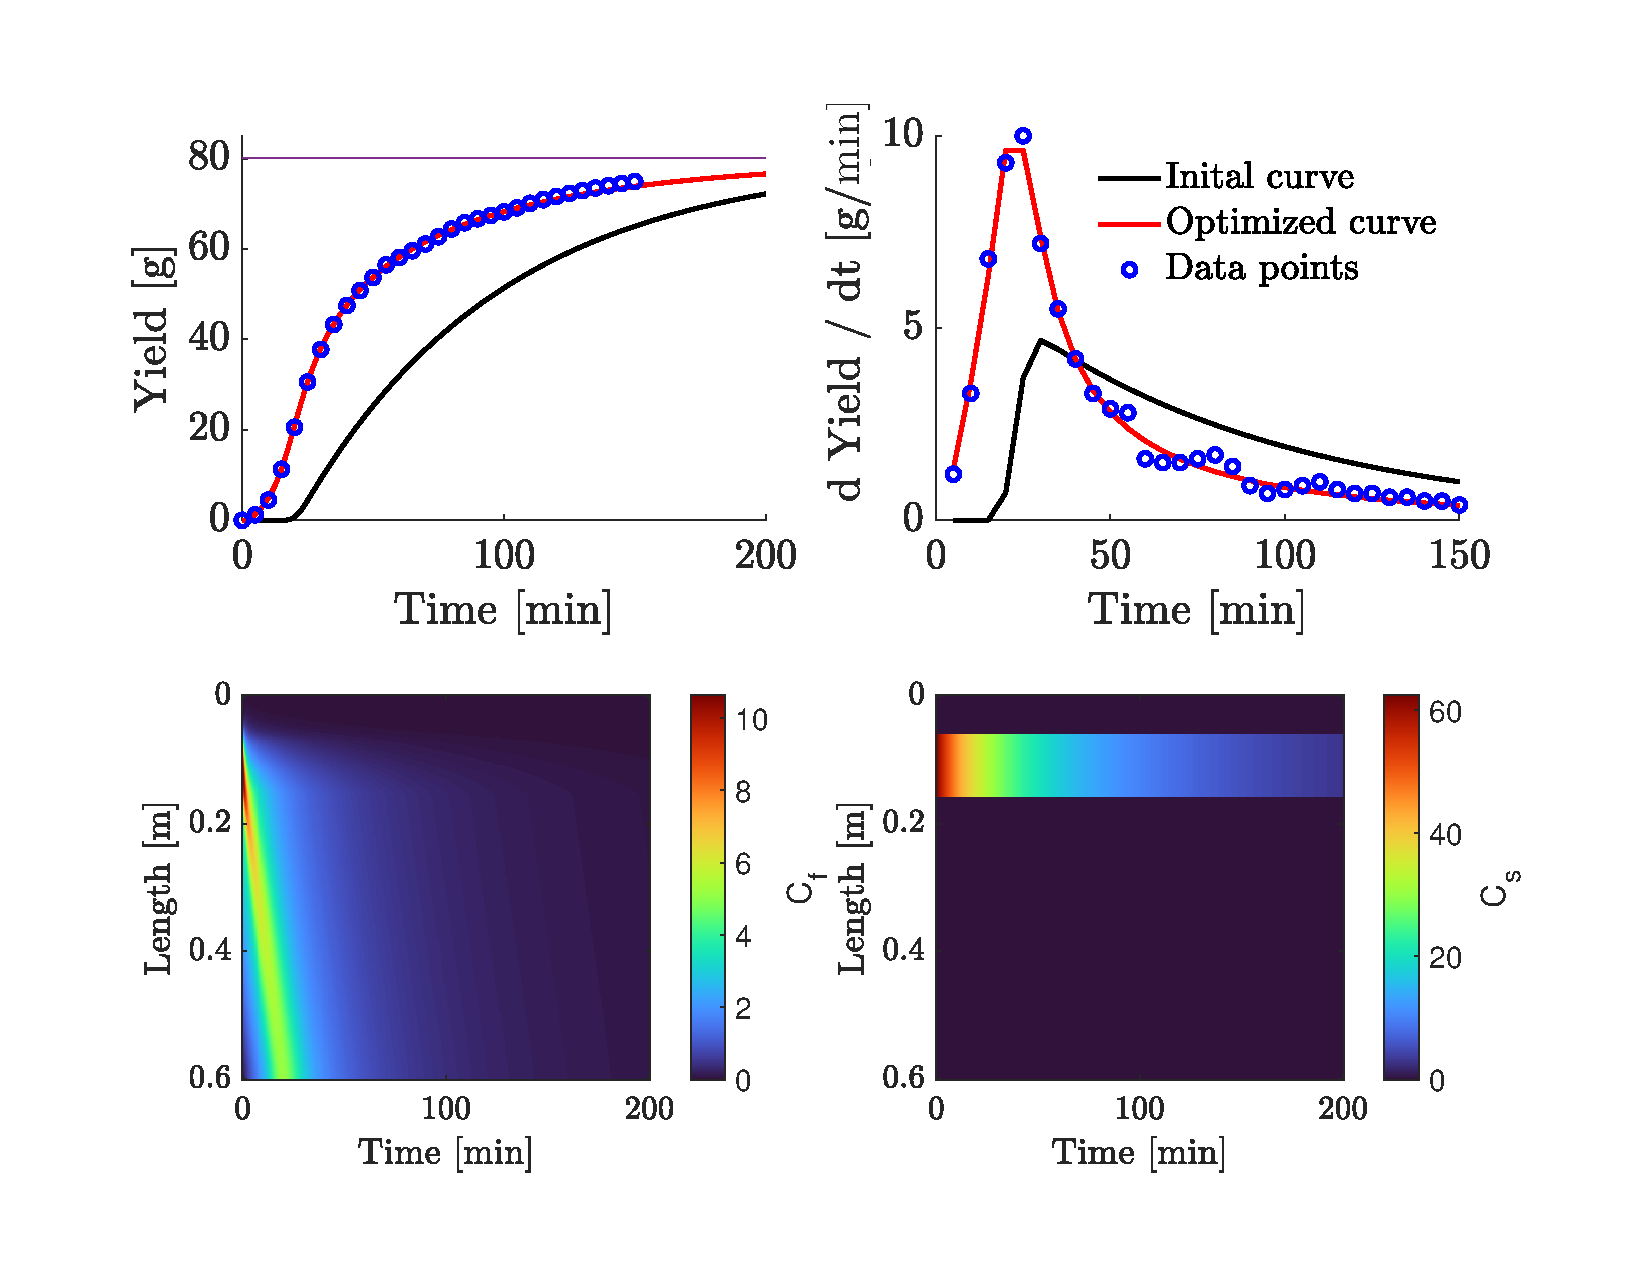
\includegraphics[trim = 2cm 10.5cm 2.5cm 1.7cm,clip,width=0.99\textwidth]{/Results_estimation/Fitting_LUKE_T50_P300.pdf}
			\caption{Experiment at $50~^\circ C$ and 300 bar}
		\end{subfigure}
		\caption{Results of parameter estimation}
		\label{fig: estimation_results}
	\end{figure}
	
\end{document}